\section{Measurement of Thermal Energy}

\begin{multicols}{2}


\section*{Specific Heat Capacity}


\subsection{Specific Heat Capacity of Liquids}

\begin{center}
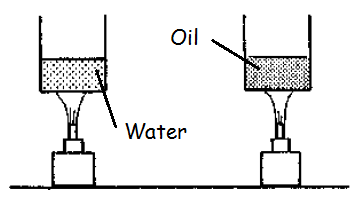
\includegraphics[width=0.4\textwidth]{./img/source/shc-liquids.png}
\end{center}

\begin{description*}
%\item[Subtopic:]{}
\item[Materials:]{}
\item[Setup:]{}
\item[Procedure:]{}
\item[Hazards:]{}
\item[Questions:]{}
\item[Observations:]{}
\item[Theory:]{}
\item[Applications:]{}
\item[Notes:]{}
\end{description*}

\subsection{Mass and Thermal Energy}

\begin{center}
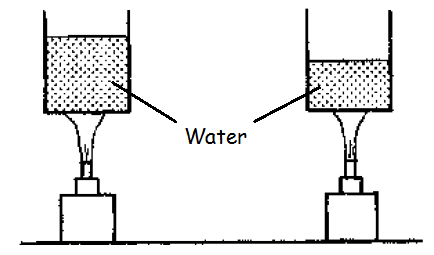
\includegraphics[width=0.4\textwidth]{./img/source/thermal-energy.png}
\end{center}

\begin{description*}
%\item[Subtopic:]{}
\item[Materials:]{}
\item[Setup:]{}
\item[Procedure:]{}
\item[Hazards:]{}
\item[Questions:]{}
\item[Observations:]{}
\item[Theory:]{}
\item[Applications:]{}
\item[Notes:]{}
\end{description*}

\subsection{The Calorimeter}

\begin{center}
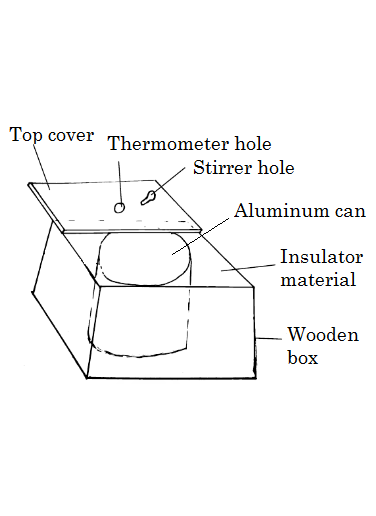
\includegraphics[width=0.4\textwidth]{./img/source/calorimeter.png}
\end{center}

\begin{description*}
%\item[Subtopic:]{}
\item[Materials:]{}
\item[Setup:]{}
\item[Procedure:]{}
\item[Hazards:]{}
\item[Questions:]{}
\item[Observations:]{}
\item[Theory:]{}
\item[Applications:]{}
\item[Notes:]{}
\end{description*}

\subsection{Determining Specific Heat Capacity of a Liquid}

%\begin{center}
%\includegraphics[width=0.4\textwidth]{./img/source/.png}
%\end{center}

\begin{description*}
%\item[Subtopic:]{}
\item[Materials:]{}
\item[Setup:]{}
\item[Procedure:]{}
\item[Hazards:]{}
\item[Questions:]{}
\item[Observations:]{}
\item[Theory:]{}
\item[Applications:]{}
\item[Notes:]{}
\end{description*}

%==================================================================================================%

\section*{Change of State}

\begin{center}
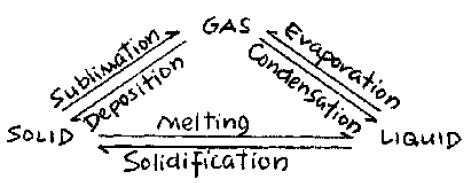
\includegraphics[width=0.4\textwidth]{./img/source/change-of-state.png}
\end{center}

%==================================================================================================%

\section*{Melting Point}


\subsection{Determining Melting Point}

\begin{center}
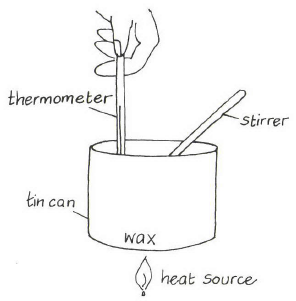
\includegraphics[width=0.4\textwidth]{./img/vso/melting-point.png}
\end{center}

\begin{description*}
%\item[Subtopic:]{}
\item[Materials:]{}
\item[Setup:]{}
\item[Procedure:]{}
\item[Hazards:]{}
\item[Questions:]{}
\item[Observations:]{}
\item[Theory:]{}
\item[Applications:]{}
\item[Notes:]{}
\end{description*}

\subsection{Pressure and Melting Point}

\begin{center}
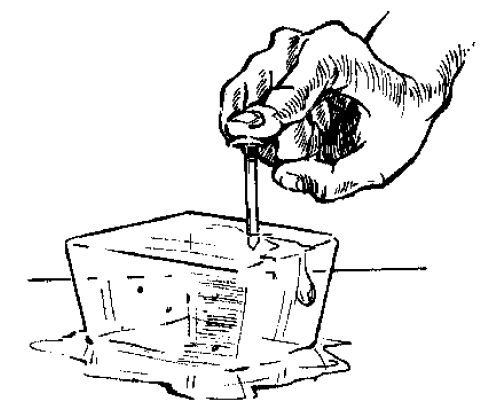
\includegraphics[width=0.4\textwidth]{./img/source/pressure-melting-point.png}
\end{center}

\begin{description*}
%\item[Subtopic:]{}
\item[Materials:]{}
\item[Setup:]{}
\item[Procedure:]{}
\item[Hazards:]{}
\item[Questions:]{}
\item[Observations:]{}
\item[Theory:]{}
\item[Applications:]{}
\item[Notes:]{}
\end{description*}

%==================================================================================================%

\section*{Boiling Point}


\subsection{Boiling at Room Temperature}

\begin{center}
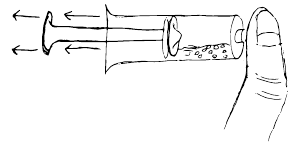
\includegraphics[width=0.4\textwidth]{./img/boiling-room-temp.png}
\end{center}

\begin{description*}
%\item[Subtopic:]{}
\item[Materials:]{}
\item[Setup:]{}
\item[Procedure:]{}
\item[Hazards:]{}
\item[Questions:]{}
\item[Observations:]{}
\item[Theory:]{}
\item[Applications:]{}
\item[Notes:]{}
\end{description*}

\subsection{Pressure Cooker}

\begin{center}
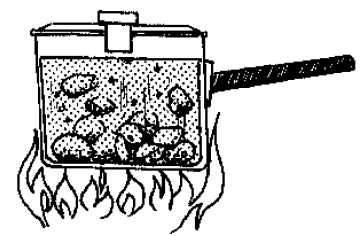
\includegraphics[width=0.4\textwidth]{./img/source/pressure-cooker.png}
\end{center}

\begin{description*}
%\item[Subtopic:]{}
\item[Materials:]{}
\item[Setup:]{}
\item[Procedure:]{}
\item[Hazards:]{}
\item[Questions:]{}
\item[Observations:]{}
\item[Theory:]{}
\item[Applications:]{}
\item[Notes:]{}
\end{description*}

\subsection{Impurities and Boiling Point}

%\begin{center}
%\includegraphics[width=0.4\textwidth]{./img/source/.png}
%\end{center}

\begin{description*}
%\item[Subtopic:]{}
\item[Materials:]{}
\item[Setup:]{}
\item[Procedure:]{}
\item[Hazards:]{}
\item[Questions:]{}
\item[Observations:]{}
\item[Theory:]{}
\item[Applications:]{}
\item[Notes:]{}
\end{description*}

%==================================================================================================%

\section*{Evaporation}


\subsection{Evaporation and Cooling}

\begin{center}
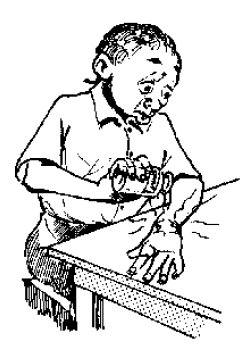
\includegraphics[width=0.4\textwidth]{./img/source/evap-cooling.png}
\end{center}

\begin{description*}
%\item[Subtopic:]{}
\item[Materials:]{}
\item[Setup:]{}
\item[Procedure:]{}
\item[Hazards:]{}
\item[Questions:]{}
\item[Observations:]{}
\item[Theory:]{}
\item[Applications:]{}
\item[Notes:]{}
\end{description*}

\subsection{Cooling Water}

\begin{center}
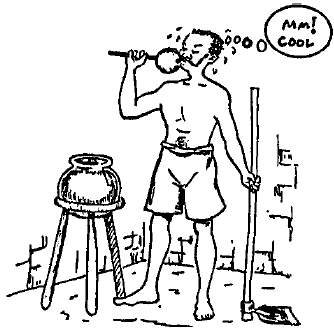
\includegraphics[width=0.4\textwidth]{./img/source/cooling-water.png}
\end{center}

\begin{description*}
%\item[Subtopic:]{}
\item[Materials:]{}
\item[Setup:]{}
\item[Procedure:]{}
\item[Hazards:]{}
\item[Questions:]{}
\item[Observations:]{}
\item[Theory:]{}
\item[Applications:]{}
\item[Notes:]{}
\end{description*}

\subsection{Latent Heat of Vaporisation}

%\begin{center}
%\includegraphics[width=0.4\textwidth]{./img/source/.png}
%\end{center}

\begin{description*}
%\item[Subtopic:]{}
\item[Materials:]{}
\item[Setup:]{}
\item[Procedure:]{}
\item[Hazards:]{}
\item[Questions:]{}
\item[Observations:]{}
\item[Theory:]{}
\item[Applications:]{}
\item[Notes:]{}
\end{description*}

\subsection{Distillation}

\begin{center}
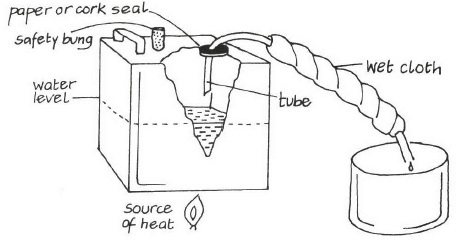
\includegraphics[width=0.4\textwidth]{./img/vso/distillation.png}
\end{center}

\begin{description*}
%\item[Subtopic:]{}
\item[Materials:]{}
\item[Setup:]{}
\item[Procedure:]{}
\item[Hazards:]{}
\item[Questions:]{}
\item[Observations:]{}
\item[Theory:]{}
\item[Applications:]{}
\item[Notes:]{}
\end{description*}

%==================================================================================================%


\end{multicols}

\pagebreak